\chapter{Ausblick}
\label{chap:ausblick}

Im Abschluss dieser Arbeit werden noch kurz offene Felder und weitere Ideen für die Zukunft diskutiert.

\paragraph{Material Graph} Auf Basis des entwickelten Rendering-Frameworks könnte in Zukunft eine Bibliothek zur semi-prozeduralen Erzeugung von Materialien entwickelt werden. Die könnte aus Bausteinen bestehen, die sich mittels eines gerichteten Graphens in Abhängigkeit zueinenader setzten lassen. Eine anschließende toplogische Sortierung der Knoten dient zur Auflösung der Abhängigkeiten. Die Bausteine könnten entweder Texturen als Basis in den Graphen importieren oder prozedural erzeugen. Weitere Bausteine filtern, kombinieren oder manipulieren auf sonstigem Wege ihre Eingangskanäle. Die Form der Definition des Rendersystems aus dieser Arbeit weißt schon eine Struktur auf, die das ermöglichen würde. Die Idee stammt aus diversen Material Editoren, wie dem des \textit{Unreal 4 Editors} (siehe \fref{fig:material-graph}) oder \textit{Shader Forge}\footnote{http://www.acegikmo.com/shaderforge/} oder \textit{Substance Designer}\footnote{https://www.allegorithmic.com/products/substance-designer}.

\begin{wrapfigure}{r}{0.5\linewidth}
\centering
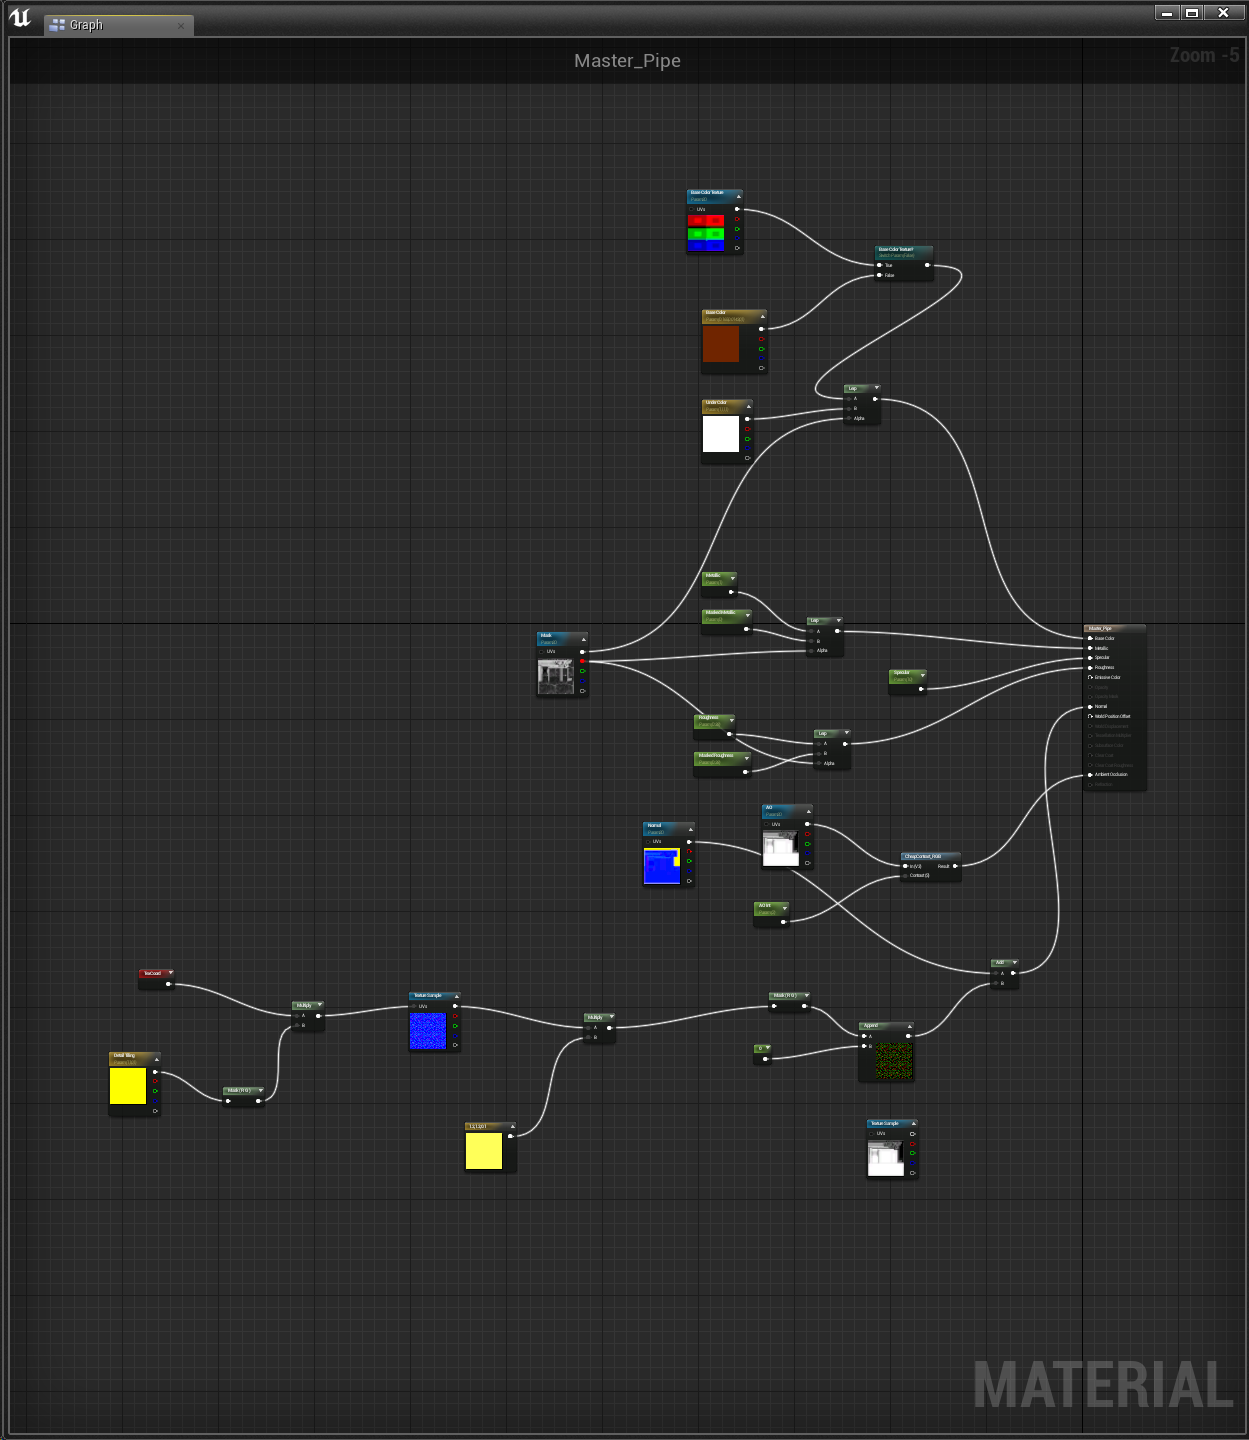
\includegraphics[width=0.5\textwidth]{ue4-material-graph}
\caption{Unreal Engine 4 \mbox{Material Graph}}\label{fig:material-graph}
\end{wrapfigure}

\paragraph{GUI-Framework}\label{sec:gui-framework} Haskell mangelt es an in ausschließlich in Haskell definierten und platformunabhängigen \acsp{GUI}. Bestehende Bindings zu \acs{GUI}-Frameworks sind oft nur unter großem Aufwand, zum Beipsiel unter Windows oder OS X, für einzurichten. Hinzu kommt, dass diese externen Frameworks imperativ gefärbt sind und deswegen oft noch funktional adaptiert werden müssen. Ein ausschließlich auf funktionalen Konzepten (z.B. \ac{FRP}\footnote{http://stud.fh-wedel.de/\~inf9912/research/20131207-info-seminar-frp-netwire/}) basierendes \acs{GUI}-Framework ohne Abhängigkeiten die sich als Hürde für Entwickler und Anwender herausstellen, brächte einige Vorteile für Akzeptanz von Haskell mit sich. Lässt sich erst einmal auf breiter Front produktive Anwendungssoftware entwickeln, die auch nicht nur hinter verschlossenen Türen verwendet wird, dürfte das weitere Aufmerksamkeit von Entwicklern auf Haskell ziehen. Oft wird von außenstehenden Entwicklern berechtigterweise angebracht, dass es wenige "`Real World"' Anwendungen von Haskell gibt oder wenn es sie gibt, sie nur versteckt hinter verschlossenen Türen existieren und nicht bewusst wahrgenommen werden, wie dies zum Beispiel bei Server-Anwendungen der Fall ist.

\paragraph{Vulkan \& SPIR-V} Zu den Kernzielen von \textit{Vulkan} gehören zum einen die Reduzierung des \acs{API}-Overheads und die Reduzierung der \ac{API} auf die modernen und wesentlichen Funktionen (\fref{sec:vulkan}) aber auch zum anderen in der Entwicklung einer expliziten \acs{API}. Sollte dies gelingen, drüfte sich der Umfang der \acs{API} deutlich reduzieren, und so könnten sich neue Möglichkeiten für die funktionale Adaptierung der Grafik-\acs{API} entwickeln. Die explizite \ac{API} könnte es zum ersten mal bei vertretbaren Aufwand ermöglichen die \ac{API} in einer relativ kompakten \ac{DSL} abzubilden. Da sich Haskell selbst sehr gut zur Definition, Parsen und Übersetzen von Sprachen eignet, könnte mit der Zwischensprache \textit{SPIR-V} sich die Möglichkeit auftun, eine (Teil-) Menge von Haskell direkt nach \textit{SPIR-V} hin zu übersetzen. Beispielsweise mittels der \acf{GHC}-\acs{API}, wie dies bei \textit{GHCJS}\footnote{https://github.com/ghcjs/ghcjs} bereits realisiert it.
